\documentclass[12pt,helvetica,a4paper,final]{iopart}
\usepackage{iopams}  
\linespread{1.375}
\usepackage{graphicx}
\usepackage[tmargin=4cm, lmargin=3cm, rmargin=3cm]{geometry}
\usepackage[breaklinks=true,colorlinks=true,linkcolor=blue,urlcolor=blue,citecolor=blue]{hyperref}
\usepackage{caption,subcaption}
\newenvironment{nstabbing}
  {\setlength{\topsep}{0pt}%
   \setlength{\partopsep}{0pt}%
   \tabbing}
  {\endtabbing}
\usepackage{subcaption}
\captionsetup[figure]{labelfont=bf,labelsep=period}
\captionsetup[subfigure]{labelfont=bf,textfont=normalfont}
\captionsetup[subfigure]{labelformat=simple}
\renewcommand\thesubfigure{(\alph{subfigure})}
\makeatletter
\newcommand*{\rom}[1]{\expandafter\@slowromancap\romannumeral #1@}
\makeatother
\setlength{\belowcaptionskip}{-3pt}
\begin{document}
\maketitle
 
\title[Solar Gravitational Waves]{Solar Gravitational Waves}
\author{ID: 2061022A. {\normalfont {\small Supervisor: Matthew Pitkin}}}
\address{School of Physics and Astronomy, University of Glasgow}
\eads{\mailto{2061022a@student.glasgow.ac.uk}}

\begin{abstract}

A direct detection of gravitational waves (GWs), as predicted by general relativity a century ago, has not been confirmed so far. As the Laser Interferometer Gravitational-wave Observatory (LIGO) detectors reach better sensitivities, a large amount of searches are directed towards detection from sources such as compact binary systems, pulsars, and supernovae. In this paper, one of the less-conventional potential sources of GWs is studied: our Sun. Existing theoretical motivation suggests that the Sun should emit low-frequency GWs due to a magnetohydrodynamic (MHD) dynamo at its core. The LIGO S6 data is used between a frequency of 100 and 300 Hz to investigate any strain signal in the detectors resulting from the Sun's GWs. Data with the same periodicity as the Sun is used for the background. The result shows a signal from the Sun that is significantly higher than the background, but more tests are needed to establish whether it is a true GW detection or not. An upper limit is further set, on the signal a GW emitted from the Sun would have between 100 and 300 Hz, which is found to be $1.215 \times 10^{22}$. 


\end{abstract}
\section{Introduction}
\subsection{LIGO and Gravitational Wave Detection}
\begin{figure}[htbp]
\begin{center}
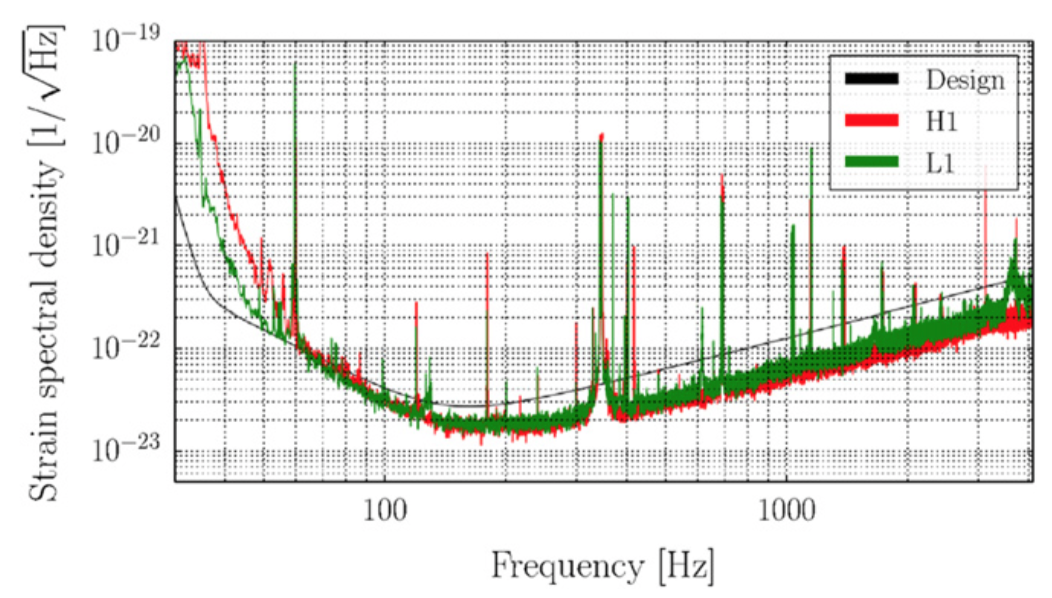
\includegraphics[width=\textwidth]{sencurve}
\caption{Sensitivity curve for LIGO S6 run as a function of frequency.}
\label{sencurve}
\end{center}
\end{figure}

GWs, distortions in space emitted from asymmetric accelerations, are one of the implications of Einstein's general relativity. A century after general relativity, searches for direct detection of GWs are still active and are currently being led by the Laser Interferometer Gravitational-wave Observatory (LIGO) Scientific Collaboration (LSC) and VIRGO Collaboration. 

\par{}
LIGO operates two detectors in Louisiana and Washington~\cite{ligo}. The gravitational-wave detector is a simple Michelson interferometer, with Fabry-P\'{e}rot cavities as its 4km interferometric arms. The laser gets reflected repeatedly making an effective length of approximately 300 km per arm. At rest, the laser from the detectors cancels out due to their phase-difference. When a GW passes through the detector, it stretches space in on direction while compressing it another perpendicular direction, resulting in a phase-difference in the interferometer that does not allow the laser reflected from the two mirrors to cancel out~\cite{kip}, and, therefore resulting in the detection of the GW. Using two separate detectors, one can point the detectors to a particular point by setting an appropriate time-delay between the two detectors~\cite{sgwb}, knowing that they travel at the speed of light. In this project, the coordinates of the Sun are used and updated over the period of the analysis to set this time-delay.
\par{}
The sixth LIGO science run data was used in this analysis, which has a maximum strain sensitivity between $10^{-22}$ and $10^{-23}$~\cite{LIGO:2012aa}. Figure~\ref{sencurve} shows the sensitivity curve (amplitude spectral density) as a function of frequency~\cite{newplot}. 

\subsection{Solar MHD Dynamo}
\begin{figure}
\begin{minipage}[c][23cm]{0.9\textwidth}
  \caption{Effect of bandpass-filtering between 100 and 300 Hz}
  \centering
  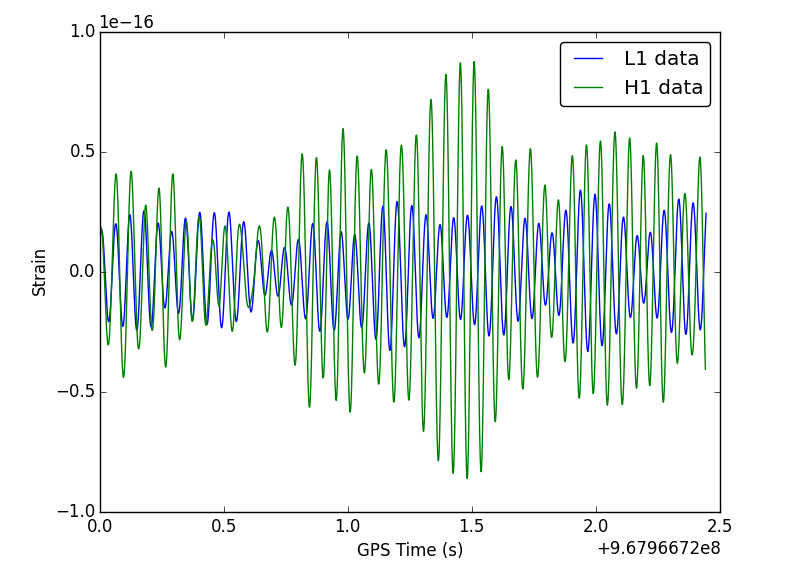
\includegraphics[width=0.95\textwidth]{L1_H1}
  \subcaption{Strain data before filtering}
  \label{figa}
   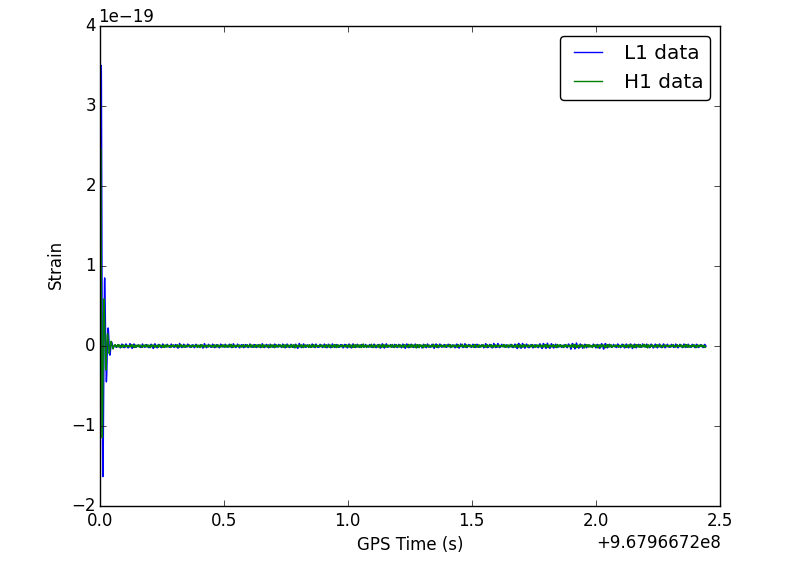
\includegraphics[width=\textwidth]{bandpass}
  \subcaption{Strain data after filtering}
  \label{figb}
\end{minipage}
\end{figure}

Most of the gravitational-wave searches so far target sources such as compact binary systems~\cite{bh1},~\cite{bh2} (black hole, neutron star, or white dwarf binaries), supernovae~\cite{supernovae}, pulsars (continuous waves)~\cite{pulsars}, and the stochastic GW background - the remnant of the big bang~\cite{sgwb},~\cite{sgwb2}. None of these S6 searches reported gravitational-wave detection. Most of the existing theoretical studies~\cite{theory2} as well as simulations~\cite{sim2},~\cite{sim}  also target such sources. In this project, we use the S6 data to study one of the less-traditional sources: the Sun.
\par{}
Winterberg recently conjectured~\cite{winterberg} that the magnetohydrodynamic (MHD) dynamo at the core of the Sun should emit GWs, albeit at a lower frequency than LIGO is most sensitive to. These GWs could theoretically show a strain signal of up to $h = ~10^{-10}$~\cite{winterberg}. Furthermore, these GWs might, themselves, be a noisy background when looking for GWs from more traditional sources that might be preventing their detection. This provides theoretical motivation for our search. 

\section{Method}

Segments of the data running both L1 (Livingston, Louisiana) and H1 (Hanford, Washington) without inconsistently large noise were used within the S6 run, which occurred from July 2009 through October 2010. The time-series data was filtered with a bandpass filter between 100 and 300 Hz to eliminate low- and high-frequency noise. Figures~\ref{figa} and~\ref{figb} illustrate a sample signal before and after this filtering, respectively, showing this effect. This filtering leaves a filter response, which appears predominantly at the start of the studied segment, figure~\ref{impulse} shows the filter response from an impulse signal, which can be seen to last a few minutes, therefore, the first 3 minutes of every segment were cut off before carrying on with the analysis.

\begin{figure}[htb]
\begin{center}
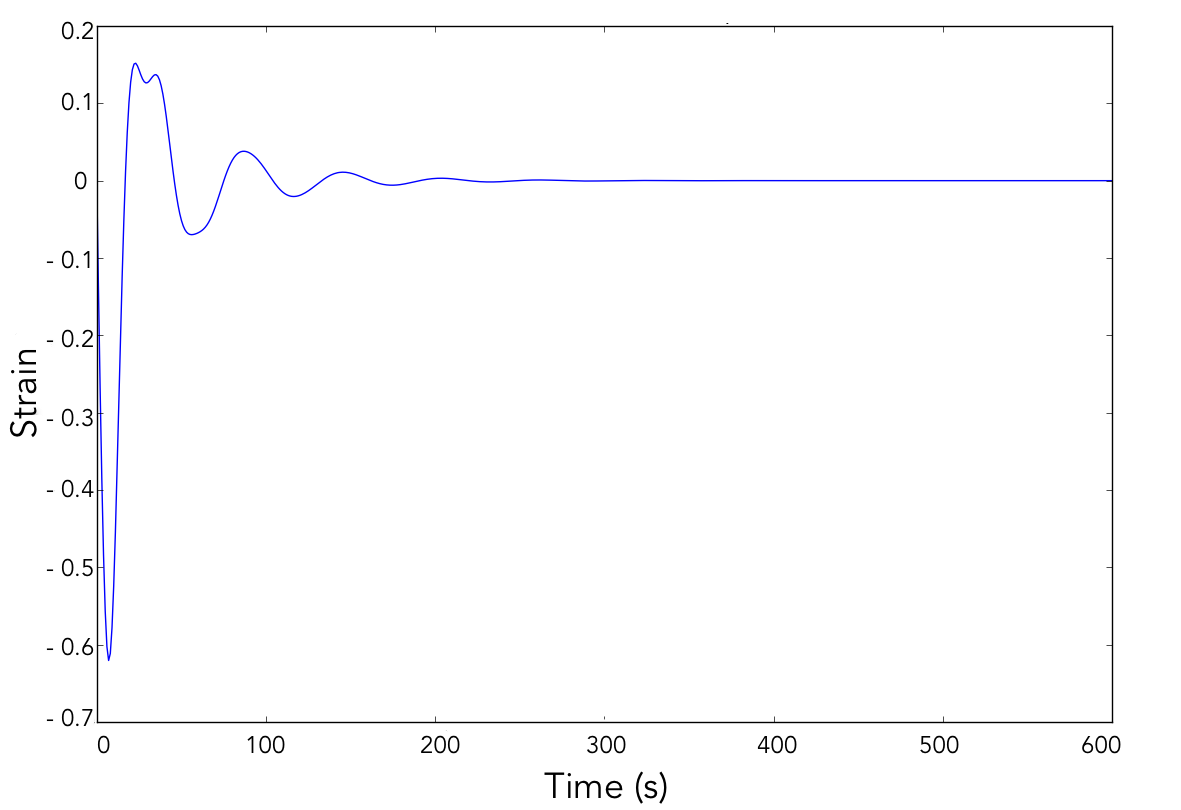
\includegraphics[width=0.9\textwidth]{impulse}
\caption{Filter response for an impulse signal}
\label{impulse}
\end{center}
\end{figure}

\par{}
The coordinates of the Sun were used to set the time-delay between the two detectors. These coordinates change, however, and therefore the time-delay should also change accordingly so that the detectors keep pointing at the Sun. Figure~\ref{tdt} shows the sinusoidal change of the time-delay for a little over a day ($10^{5}$ seconds). The largest allowable change of coordinates, with regards to the sensitivity of the detector, was chosen such that the change in time-delay is always smaller than $0.05 \over \omega$ where $\omega$ is the angular frequency, from that it follows that the maximum allowable change in time-delay is 0.0000265. Figure~\ref{ddt} shows a comparison of different durations to update the coordinates at, to test the change in time-delay, and illustrates why choosing 30-second segments is thus a legitimate choice. 
\begin{figure}[htb]
\begin{center}
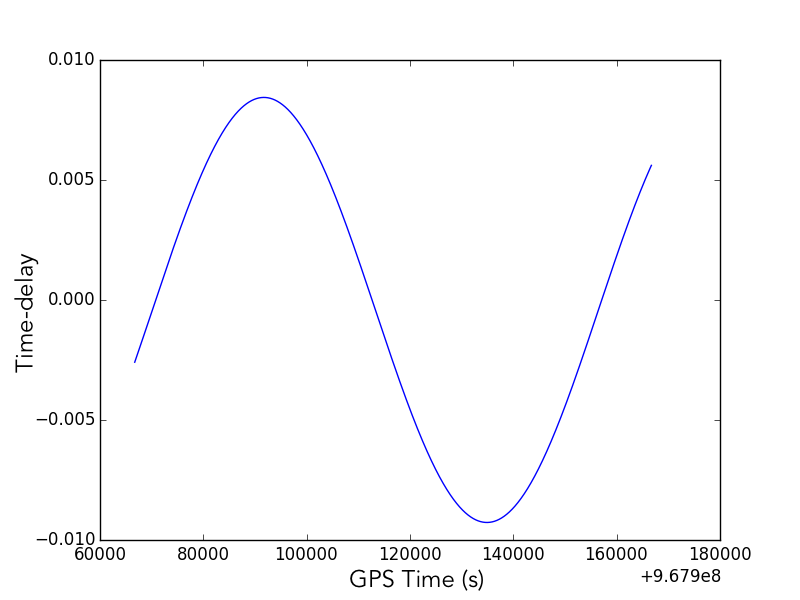
\includegraphics[width=\textwidth]{t_dt}
\caption{Time-delay over approx. 28 hours ($10^{5}$ seconds)}
\label{tdt}
\end{center}
\end{figure}
\par{} 
The same data with 100 different time-delays pointing where the position of the Sun was at different times (10, 20, 30, etc. minutes before) were used for the background signal. This might potentially eliminate false-positives as the background now has the same periodicity as the Sun.

\begin{figure}[htb]
\begin{center}
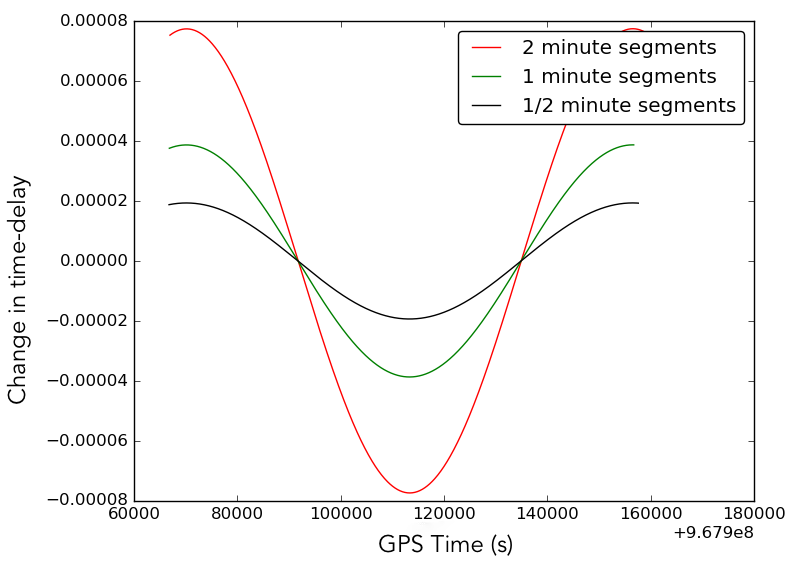
\includegraphics[width=0.9\textwidth]{ddt}
\caption{Change of time-delay over a day for several segments. The selected segment duration needs to be less than 0.000026 to keep the detectors in sync. 30 seconds was chosen as the 'coordinates update time'.}
\label{ddt}
\end{center}
\end{figure}\par{}
% talk about figure
\par{}
The dot product of the 30-second segments for the two detectors were then taken to cross-correlate their signals, for both the Solar and background signals, to compare them and look for GW detection.

\section{Results}
  \begin{figure}
  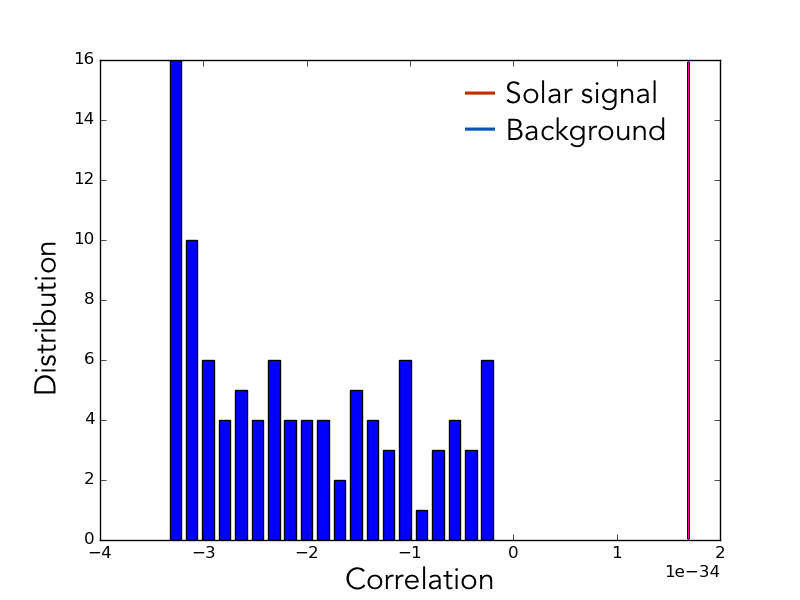
\includegraphics[width=\textwidth]{strain1}
  \caption{Comparison between the Solar signal (single value) and 100 (plotted as a histogram) background data points, summed up over the entire 775.5 hours used from the S6 data (July 2009 - October 2010).}
  \label{strain}
  \end{figure}
To search for a GW signal, the data from the two LIGO detectors was cross-correlated and summed up as follows:
\bigskip \bigskip \bigskip \bigskip \bigskip \bigskip

\begin{equation}
cor = \sum^N h_{L1}(t) \cdot \sum^N h_{H1}(t)
\label{eq:cor}
\end{equation}
where:
\begin{nstabbing}
\phantom{$D_{n40}\ $}\= \kill
N\> is the number of data points: $ \frac { \textrm{the duration}}{\textrm{the time-spacing}},$\\
h\> is the strain signal for H1 and L1 as a function of time.\\
\end{nstabbing}
The duration of the entire data used sums up to 775.5 continuous hours, and the time-spacing is $2.44140625 \times 10^{-4}$ resulting in an N = 3176448. Using equation~\ref{eq:cor}, for both the Solar signal and the background, figure~\ref{strain} was produced with the background plotted as a histogram and the Solar signal represented by the red, vertical line. It can be seen from the plot that the signal from the Sun is indeed higher than the background, with potential for GWs to be detected. The background can be seen to be biased towards negative values. Without further tests and checks, however, no GW detection claim can be made. This result was found towards the end of the project and we plan to continue testing it further soon. 


Using these results, an upper limit on GWs emitted from the Sun in the frequency range of 100 to 300 Hz can be estimated as follows:
\begin{eqnarray}
\label{uplim}
h_{max} & = \sqrt{\frac{ \sum^N h_{L1}(t) \cdot \sum^N h_{H1}(t)}{N}} \\[10pt] \nonumber
& = \sqrt{\frac{ N^2 \, (h_{L1}(t) \cdot  h_{H1}(t))}{N}} \\[10pt] \nonumber
& = \sqrt{ N \, (h_{L1}(t) \cdot  h_{H1}(t))} \nonumber
\end{eqnarray}

Following equation~\ref{uplim} we find that, in this case, the upper limit is $1.215 \times 10^{22}$.
This estimation of the upper limit ignores the noise in the detectors, and a more rigorous estimation can be made (see upper limit estimations in e.g.~\cite{bh1} and~\cite{bh2}).

\section{Conclusion}
Gravitational wave research has come a long way in terms of theory and detector sensitivity, While most of the experimental and theoretical searches and simulations of GWs has so far targeted sources such as compact binary systems, pulsars, supernovae and the stochastic GW background, any asymmetric acceleration will emit gravitational waves. An MHD dynamo at the core of the Sun should emit GWs, and, albeit at a lower frequency than LIGO's more-sensitive bands, still motivates a search for GWs from the Sun. This project uses the LIGO S6 data when both detectors were running with low noise. The data is filtered using a bandpass filter to frequencies between 100 and 300 Hz, and the time-delay between the two LIGO detectors is used to point the detectors at the Sun. This time-delay is updated every 30 seconds according to the coordinates of the Sun. 100 other points were used as a background signal with the same periodicity of the Sun. The signals from the two LIGO detectors were then cross-correlated and summed over the 775.5 hours, and the resulting signal from the Sun appears significantly higher than that of the background - which seems to be biased towards negative values. Several checks and tests, however, are needed to establish whether it is a true GW signal or not, and to check whether the background data is correlated or biased. An upper limit on GW strain signal, was also estimated from the results and is found to be $1.215 \times 10^{22}$.
\section*{References}% !TEX root =  
\begin{flushleft}
\bibliographystyle{unsrt}
\bibliography{biblio}
\end{flushleft}
\end{document}